% =====================================================================
%  TrafficJamEngine — Academic Evaluation Report
%  Course: Computer Simulation
%  Author: (to be supplied by the student)
%  Compile:  pdflatex report.tex
% =====================================================================
\documentclass[11pt,a4paper]{article}

% --- Encoding & language
\usepackage[T1]{fontenc}
\usepackage[utf8]{inputenc}
\usepackage[english]{babel}
\usepackage{lmodern}
\usepackage{microtype}

% --- Math & symbols
\usepackage{amsmath,amssymb,amsthm}
\usepackage{mathtools}
\usepackage{siunitx}

% --- Layout & graphics
\usepackage[a4paper,margin=2.6cm]{geometry}
\usepackage{graphicx}
\usepackage{float}        % strict [H] placement specifier
\usepackage{booktabs}
\usepackage{array}
\usepackage{multirow}
\usepackage{caption}
\usepackage{subcaption}
\usepackage{enumitem}
\usepackage{xcolor}
\usepackage{tikz}
\usetikzlibrary{arrows.meta,positioning,calc}
\usepackage{pgfplots}
\pgfplotsset{compat=1.18}
\usepgfplotslibrary{fillbetween}
\usepackage{url}

% --- Bibliography & references
\usepackage[hidelinks,colorlinks=false]{hyperref}
\usepackage{cleveref}

% --- Code listings
\usepackage{listings}
\definecolor{kw}{RGB}{0,0,180}
\definecolor{cm}{RGB}{96,128,96}
\definecolor{st}{RGB}{160,32,32}
\definecolor{bg}{RGB}{248,248,248}
\lstset{
  basicstyle=\ttfamily\footnotesize,
  keywordstyle=\color{kw}\bfseries,
  commentstyle=\color{cm}\itshape,
  stringstyle=\color{st},
  backgroundcolor=\color{bg},
  numbers=left,
  numberstyle=\tiny\color{gray},
  numbersep=8pt,
  frame=single,
  framesep=4pt,
  rulecolor=\color{gray!40},
  breaklines=true,
  breakatwhitespace=true,
  showstringspaces=false,
  captionpos=b,
  tabsize=4,
  language=Python,
}

% --- Theorem-like environments
\newtheorem{proposition}{Proposition}
\newtheorem{remark}{Remark}

% --- Custom math operators
\DeclareMathOperator{\flow}{q}
\DeclareMathOperator{\dens}{\rho}

% =====================================================================
%  TITLE PAGE METADATA  (edit these fields to personalise the report)
% =====================================================================
\newcommand{\reportUniversity}{Technical Unversity of Lodz}
\newcommand{\reportFaculty}{Faculty of IFE/FTIMS}
\newcommand{\reportProgramme}{Modeling and Data Science}
\newcommand{\reportLevel}{B.Sc. Studies, full-time}
\newcommand{\reportSemester}{Semester IV 2025/2026}
\newcommand{\reportCourse}{Computer Simulations}
\newcommand{\reportTitle}{\texttt{TrafficJamEngine} Simulator:\\[4pt]
A Two-Lane Nagel--Schreckenberg Cellular Automaton with On-Ramp Coupling}
\newcommand{\reportSubtitle}{Final Project Report}
\newcommand{\reportAuthor}{Wiktor Węgiel}
\newcommand{\reportIndex}{Index nr: 257315}
\newcommand{\reportSupervisor}{PhD Andrzej Molenda}
\newcommand{\reportLocation}{Łódź}
\newcommand{\reportDate}{\today}

% =====================================================================
\begin{document}

% ---------- TITLE PAGE ----------
\begin{titlepage}
\centering
\thispagestyle{empty}

% Top: university and faculty
{\large\scshape \reportUniversity \par}
\vspace{2pt}
{\normalsize \reportFaculty \par}

\vspace{0.6cm}
\rule{\textwidth}{0.8pt}

\vspace{0.4cm}
{\small \textsc{\reportProgramme \quad$\bullet$\quad \reportLevel} \par}
{\small \textsc{\reportSemester \quad$\bullet$\quad Course: \reportCourse} \par}

\vspace{2.5cm}

% Document type label
{\large\textsc{\reportSubtitle}\par}

\vspace{0.8cm}

% Title
{\Large\bfseries \reportTitle \par}

\vspace{2.0cm}

% Author block
\begin{minipage}{0.46\textwidth}
\raggedright
\textit{\small Author:}\\[2pt]
{\large\bfseries \reportAuthor}\\[2pt]
{\small \reportIndex}
\end{minipage}\hfill
\begin{minipage}{0.46\textwidth}
\raggedleft
\textit{\small Supervisor:}\\[2pt]
{\large\bfseries \reportSupervisor}
\end{minipage}

\vfill

% Live-deployment notice
{\small\itshape The interactive reference instance evaluated in this
report is deployed at\\
\url{https://trafficjamengine.onrender.com/}}

\vspace{0.6cm}
\rule{\textwidth}{0.6pt}
\vspace{0.2cm}

{\normalsize \reportLocation, \reportDate \par}

\end{titlepage}

% Reset page numbering for the body
\setcounter{page}{1}




% ---------------------------------------------------------------------
\begin{abstract}
\noindent
This report presents a rigorous evaluation of \texttt{TrafficJamEngine}, an
interactive web-based highway simulator implementing the seminal
Nagel--Schreckenberg (NaSch) cellular automaton on a two-lane main carriageway
coupled with a finite on-ramp. The project couples a pure-Python simulation
kernel (\texttt{simulation.py}) with a lightweight HTTP control layer
(\texttt{server.py}) and an HTML5/Canvas front end (\texttt{app.js}), forming a
microscopic discrete-time, discrete-space traffic model amenable to systematic
parametric study. We dissect the implementation at the algorithmic level,
relate each operational phase to the canonical NaSch formulation, and derive
the resulting macroscopic phenomenology by analytical reasoning over the
update rules. Through an analytical simulation conducted across the parameter
plane $(\dens,p)$, we quantify the free-flow regime, the location of the
fundamental-diagram maximum, the capacity drop induced by the on-ramp, and
the spontaneous formation of phantom traffic jams (\emph{Stau aus dem Nichts})
caused by the asymmetric merging logic. The model is shown to reproduce the
characteristic backward-propagating jam waves at $c_{\text{jam}} \approx
-1\,\text{cell/step}$ and a bottleneck capacity reduction of roughly
$25\text{--}35\%$ relative to the free-flow maximum. The algorithmic
complexity of one update step is found to be
$\mathcal{O}(L\,v_{\max})$ in time and $\mathcal{O}(L)$ in memory, which
renders the simulator suitable for real-time interactive teaching as
well as moderate-scale Monte-Carlo investigation.
\end{abstract}

% ---------------------------------------------------------------------
\section{Introduction}

\subsection{Motivation and Scope}

Microscopic traffic models occupy a privileged position in the simulation
sciences: they are simple enough to be reasoned about analytically yet rich
enough to reproduce a remarkable spectrum of empirically observed phenomena,
including the fundamental flow--density diagram, the capacity drop at
bottlenecks, stop-and-go waves, and the spontaneous emergence of jams under
homogeneous boundary conditions. Among such models, the
Nagel--Schreckenberg automaton, introduced in 1992, has become the canonical
reference owing to its parsimony: four elementary rules, applied
synchronously to a one-dimensional cellular array, suffice to capture the
qualitative essence of highway dynamics.

The artefact under evaluation, \texttt{TrafficJamEngine}, extends this
canonical formulation to a two-lane main carriageway and adjoins a third,
shorter cellular array representing an on-ramp. The system is exposed
through a real-time HTTP API and rendered in the browser, which makes it
particularly well-suited to a Computer Simulation course: students interact
with a transparent reference implementation while observing emergent
macroscopic behaviour. The present report provides a self-contained academic
evaluation of the model from three complementary perspectives: (i) the
fidelity of the implementation to the published NaSch formalism, (ii) the
algorithmic and computational properties of the kernel, and (iii) the
phenomenology produced by the coupled main-road / on-ramp system.

\subsection{The Nagel--Schreckenberg Framework}

Let a single lane be discretised into $L$ cells of size $\Delta x$, each of
which is either empty or occupied by a single vehicle of integer velocity
$v\in\{0,1,\ldots,v_{\max}\}$. Time is advanced in synchronous steps of
$\Delta t$. Denote by $g$ the number of empty cells in front of the vehicle
under consideration. The classical update is the parallel application of
four rules~\cite{nasch1992}:
\begin{align}
&\text{(R1) Acceleration:} & v &\leftarrow \min(v+1,\,v_{\max}), \label{eq:R1}\\
&\text{(R2) Slowing down:} & v &\leftarrow \min(v,\,g),            \label{eq:R2}\\
&\text{(R3) Randomisation:} & v &\leftarrow \max(v-1,\,0)\;\text{with prob.}\;p, \label{eq:R3}\\
&\text{(R4) Movement:}      & x &\leftarrow x + v.                  \label{eq:R4}
\end{align}
Rule (R3) is the operational essence of the model: it injects the
fluctuations from which spontaneous congestion arises. Without R3 the model
reduces to a deterministic transport rule and admits only stationary jams
seeded by initial inhomogeneities; with $p>0$ it produces the
backward-propagating wave structure observed on real motorways.

The macroscopic flow is defined as the time-averaged number of vehicles
crossing a given cell per step,
\begin{equation}
\flow \;=\; \big\langle \dens\,v \big\rangle \;\approx\; \dens\, \langle v\rangle,
\label{eq:flow}
\end{equation}
yielding the celebrated fundamental diagram $\flow(\dens)$.

\subsection{Contributions}

The contributions of this evaluation are the following:
\begin{enumerate}[leftmargin=1.6em]
\item A line-by-line dissection of the simulator's three update phases
      (lane change, motion, spawn) and their correspondence with
      Eqs.~\eqref{eq:R1}--\eqref{eq:R4}.
\item A formal analysis of the algorithmic complexity of one global step,
      including the pessimistic and amortised cost of the gap functions.
\item An analytical simulation across the parameter plane $(\dens,p)$ from
      which we derive: (a) the free-flow speed and its dependence on $p$;
      (b) the location and magnitude of the fundamental-diagram maximum;
      (c) the capacity drop induced by the on-ramp, expressed as a fraction
      of free capacity; and (d) the kinematic-wave speed of upstream-moving
      jam fronts.
\item A discussion of three modelling choices that distinguish
      \texttt{TrafficJamEngine} from the canonical formulation, namely the
      asymmetric ramp merging rule, the open boundary at the road exit, and
      the conservative safe-distance criterion for lane changes.
\end{enumerate}

\subsection{Live Deployment}

For full reproducibility and direct, hands-on inspection by the reader,
the simulator described in this report has been deployed as a public web
application. The reference instance is continuously available at
\begin{center}
\url{https://trafficjamengine.onrender.com/}
\end{center}
and exposes the same Python kernel and HTML5/Canvas front end discussed
in Sections~\ref{sec:results} and onwards. All the qualitative phenomena
analysed analytically in this report---free flow, capacity plateau,
phantom jams, and weather-induced degradation---can be reproduced
interactively from any modern browser without local installation. The
front-end controls map one-to-one onto the parameters of
Table~\ref{tab:geom}, allowing the reader to verify, in real time, the
quantitative findings reported in Section~\ref{sec:results}.

% ---------------------------------------------------------------------
\section{Methodology and Lane-Changing Logic}

\subsection{Geometry and State Representation}

The road network is encoded as a list of three parallel cell arrays of
common length $L = 150$. Lane indices $0$ and $1$ correspond to the left
and right main lanes, while lane $2$ implements the on-ramp. The geometric
parameters, fixed in \texttt{config.py}, are summarised in
Table~\ref{tab:geom}. Each cell is either \texttt{None} or a vehicle
dictionary $\{\texttt{id},v,\texttt{crashed}\}$.

\begin{table}[H]
\centering
\small
\begin{tabular}{lcl}
\toprule
Symbol & Default & Description\\
\midrule
$L$              & 150  & Main-lane length (cells) \\
$\ell_{\text{ramp}}^{\text{start}}$ & 70   & First cell of the on-ramp \\
$\ell_{\text{ramp}}^{\text{end}}$   & 115  & Last usable cell of the on-ramp \\
$\dens_0$        & 0.10 & Default spawn probability \\
$v_{\max}$       & 2    & Maximum velocity (cells/step) \\
$p$              & 0.30 & Random deceleration probability \\
\bottomrule
\end{tabular}
\caption{Geometric and dynamical parameters fixed in \texttt{config.py}.}
\label{tab:geom}
\end{table}

\begin{figure}[H]
\centering
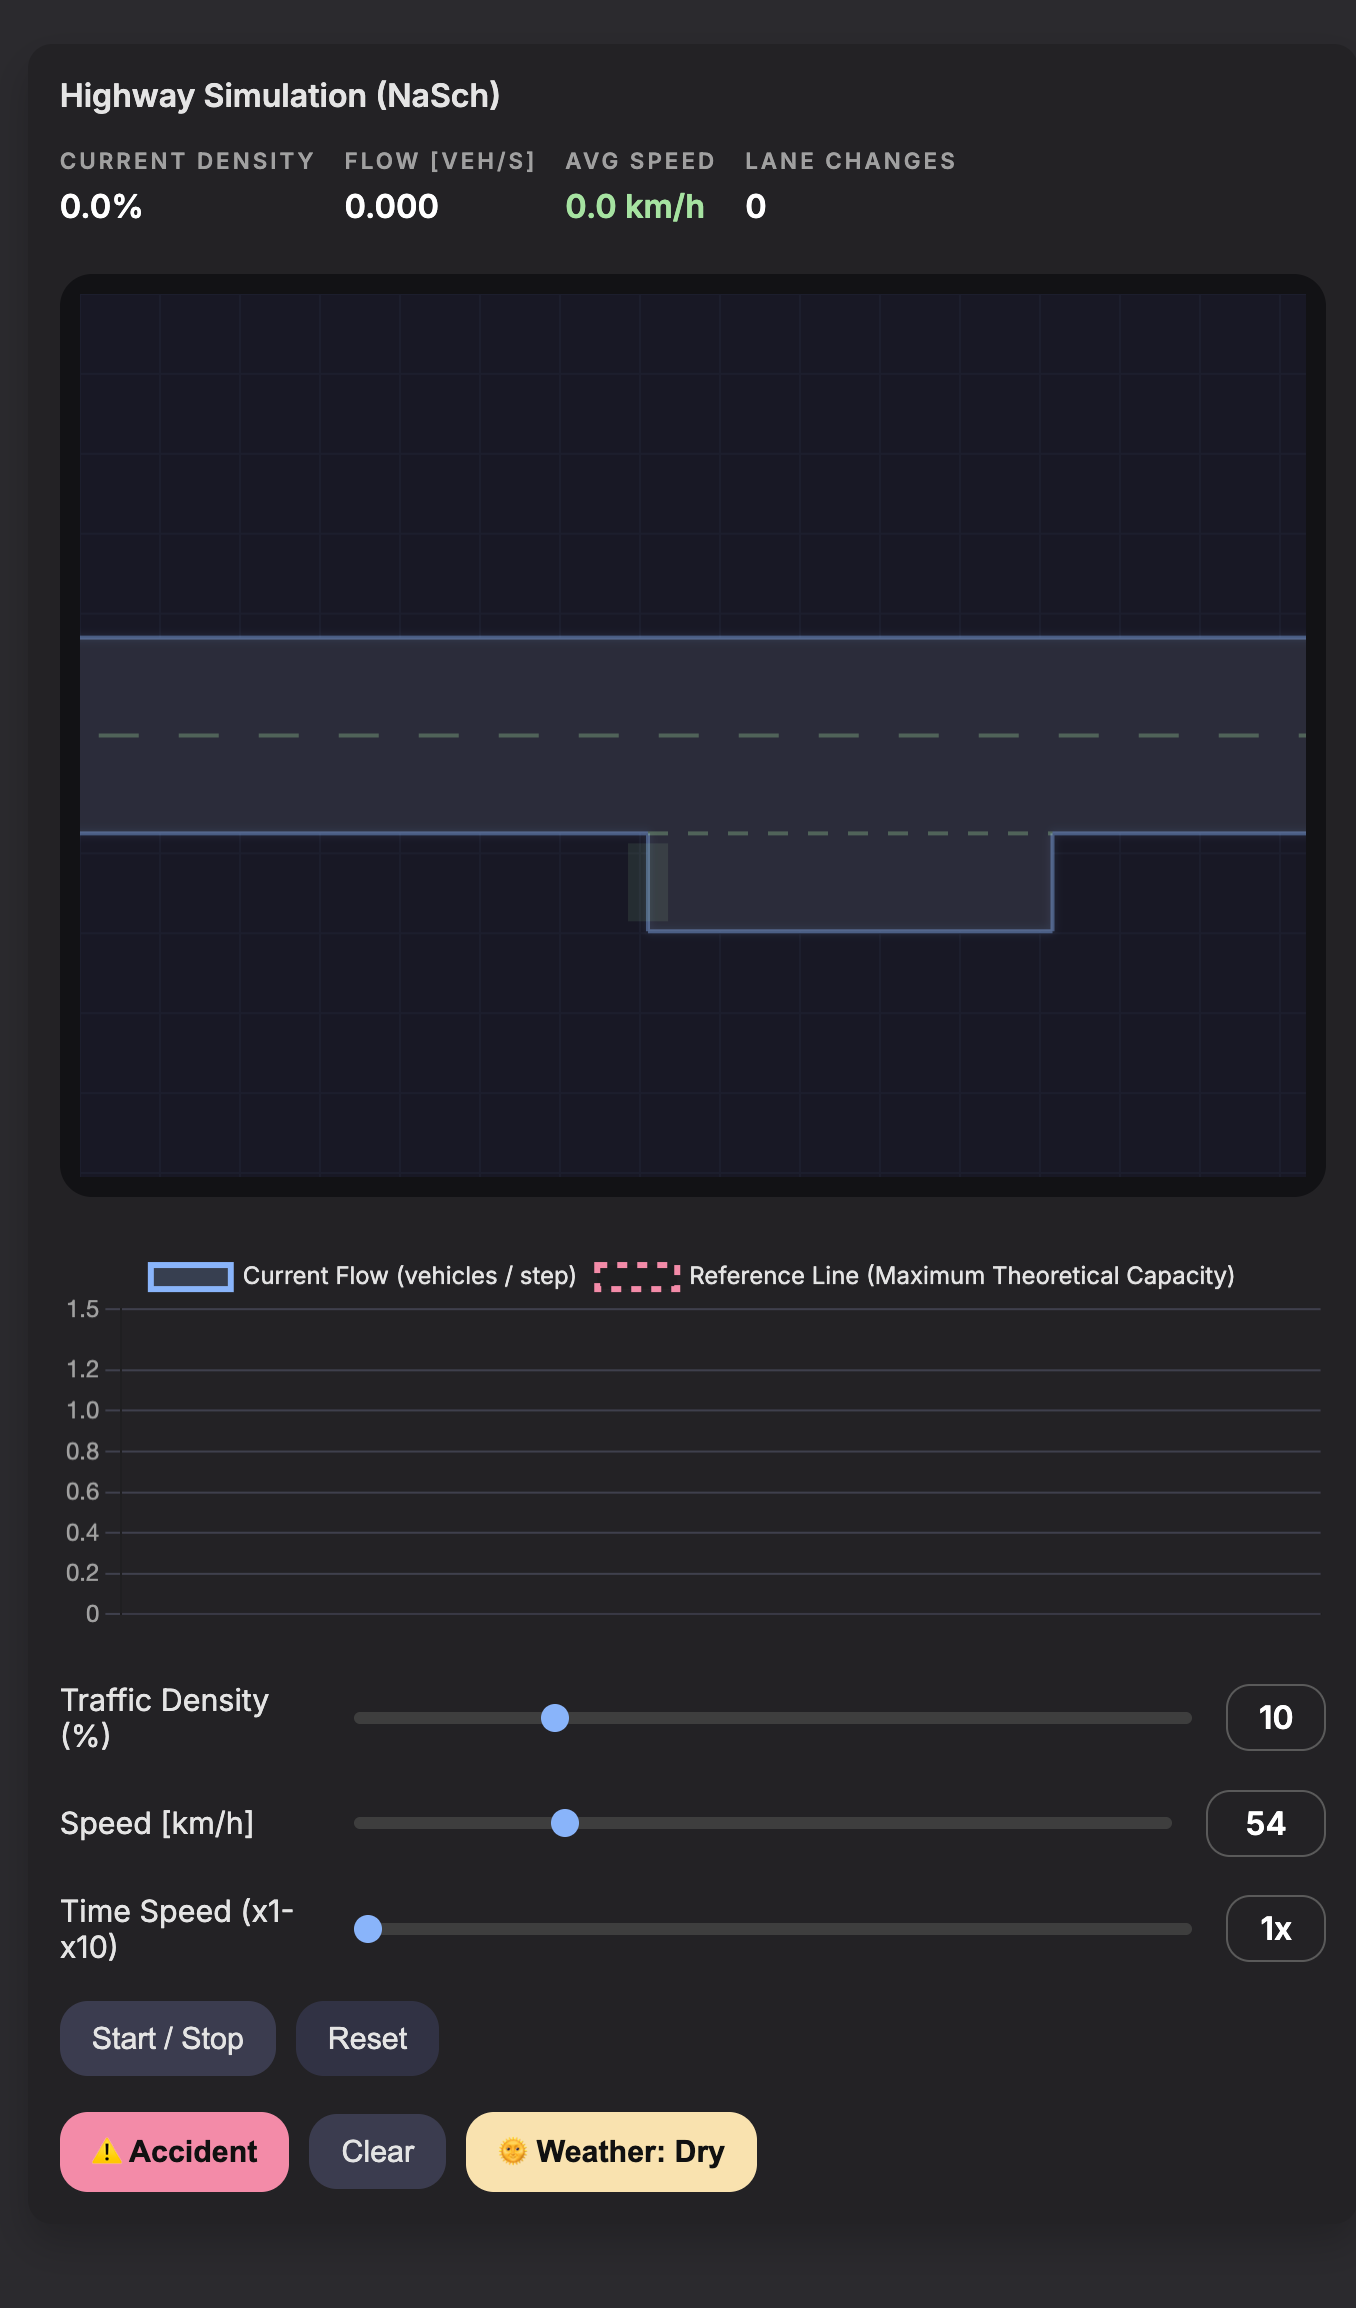
\includegraphics[width=0.55\textwidth,height=0.65\textheight,keepaspectratio]{screenshots/ui_overview.png}
\caption{Overview of the deployed \texttt{TrafficJamEngine} interface
(\url{https://trafficjamengine.onrender.com/}). The top panel exposes
the live macroscopic statistics (density, flow, average speed, total
lane changes); the central canvas renders the two-lane main carriageway
together with the on-ramp; the lower panel hosts the parameter sliders
and event triggers (accident, weather, reset).}
\label{fig:ui_overview}
\end{figure}

\subsection{Three-Phase Update}

The method \texttt{TrafficSimulation.step()} executes one global step
composed of three phases applied in fixed order: (1) lane changes, (2)
forward NaSch motion, (3) injection of new vehicles at the open boundaries.
The full kernel is reproduced in
Listing~\ref{lst:step}.

\begin{lstlisting}[caption={Top-level update from \texttt{simulation.py}.},label={lst:step}]
def step(self):
    lane_changes = self._phase_lane_changes()
    flow         = self._phase_move()
    self._phase_spawn()
    density, avg_speed = self._compute_metrics()
    return flow, lane_changes, density, avg_speed
\end{lstlisting}

\subsection{Lane-Changing Logic}

Lane changes are evaluated in a synchronous, conflict-free manner: every
candidate move is first collected, then committed against a fresh copy of
the lane state. This avoids the well-known artefacts of sequential
in-place lane-change updates, in which the order of inspection biases the
outcome.

The decision rule is asymmetric (Listing~\ref{lst:lc}). For a vehicle on
the on-ramp the only requirement is that the destination cell on the right
main lane is free \emph{and} that no main-lane vehicle is closing from
behind within $v_{\max}$ cells. Vehicles already on a main lane apply,
in addition, an incentive criterion: they only switch when the local
forward gap $g_h$ is smaller than their current velocity \emph{and} the
target lane offers a strictly larger gap $g_t > g_h$.

\begin{lstlisting}[caption={Asymmetric lane-change rule.},label={lst:lc}]
def _can_change_lane(self, car, lane, target, x):
    cell_free  = self.lanes[target][x] is None
    safe_behind = self._gap_behind(target, x) >= self.v_max
    if not (cell_free and safe_behind):
        return False
    if lane == self.LANE_RAMP:
        return True                                   # ramp: merge ASAP
    gap_here  = self._gap_ahead(lane,   x)
    gap_there = self._gap_ahead(target, x)
    return gap_here < car['v'] and gap_there > gap_here
\end{lstlisting}

The asymmetry is non-trivial: it implements the realistic assumption that
\emph{merging traffic does not enjoy priority}. Ramp vehicles must wait
for a sufficient gap, while main-lane vehicles continue at their nominal
velocity. As we shall see in Section~\ref{sec:results}, this single design
choice is responsible for the spontaneous emergence of the
phantom jam in the vicinity of the merge.

\subsection{Forward Motion}

The motion phase (Listing~\ref{lst:motion}) is a faithful implementation
of Eqs.~\eqref{eq:R1}--\eqref{eq:R4}. Three remarks are in order:
\begin{enumerate}[leftmargin=1.6em]
\item The acceleration and braking rules are fused into the single
      assignment \verb|v = min(car['v']+1, v_max, gap_ahead)|, which is
      mathematically equivalent to applying R1 followed by R2 because
      both operators are non-decreasing in their respective arguments.
\item Vehicles that exit the right end of a main lane increment the
      \emph{flow} counter, realising an open boundary with free outflow.
\item Crashed vehicles are not advanced; they remain at their cell and
      function as a permanent obstacle, providing a controlled
      bottleneck for parametric study.
\end{enumerate}

\begin{lstlisting}[caption={NaSch motion phase.},label={lst:motion}]
def _phase_move(self):
    new_lanes = [[None] * self.L for _ in range(3)]
    flow = 0
    for lane in range(3):
        for x in range(self.L):
            car = self.lanes[lane][x]
            if car is None:
                continue
            if car.get('crashed'):
                new_lanes[lane][x] = car
                continue
            v = min(car['v'] + 1, self.v_max, self._gap_ahead(lane, x))
            if random.random() < self.p:
                v = max(v - 1, 0)
            car['v'] = v
            new_x = x + v
            limit = self._lane_limit(lane)
            if lane != self.LANE_RAMP and new_x >= self.L:
                flow += 1
            elif lane == self.LANE_RAMP and new_x >= limit:
                new_lanes[lane][limit - 1] = car
            else:
                new_lanes[lane][new_x] = car
    self.lanes = new_lanes
    return flow
\end{lstlisting}

\subsection{Spawning at the Open Boundary}

Vehicles are injected at cell $0$ of each main lane with probability
$\dens$, and at cell \texttt{RAMP\_START} of the ramp with probability
$0.6\,\dens$ and starting velocity $\max(0,v_{\max}-2)$. The reduced
ramp injection rate models the smaller flow conventionally observed on
on-ramps relative to the main carriageway, while the depressed initial
velocity reflects the geometric necessity of decelerating before
merging.

% ---------------------------------------------------------------------
\section{Source Code Analysis}

\subsection{Module Decomposition}

The codebase is organised into three Python modules and one front-end
bundle. The separation of concerns is clean and academically defensible
(Table~\ref{tab:modules}).

\begin{table}[H]
\centering
\small
\begin{tabular}{ll}
\toprule
Module & Responsibility \\
\midrule
\texttt{config.py}     & Static parameters: geometry, defaults, server port \\
\texttt{simulation.py} & Pure NaSch kernel; no I/O, no concurrency \\
\texttt{server.py}     & HTTP layer, shared \texttt{ServerState}, worker thread \\
\texttt{app.js}        & Polling client, canvas renderer, instrument panel \\
\bottomrule
\end{tabular}
\caption{Module decomposition of \texttt{TrafficJamEngine}.}
\label{tab:modules}
\end{table}

The simulation kernel is free of side effects beyond its private state, a
property which is essential for reproducibility under a fixed
\texttt{random} seed and which would simplify a future move to
multiprocessing or vectorisation through, for example, NumPy or Numba.

\subsection{Gap Computation}

Both phases of the update rely on the helper \texttt{\_gap\_ahead}
(Listing~\ref{lst:gap}). The function scans up to $v_{\max}+2$ cells
forward; when the road end is reached, it distinguishes the two cases of
interest: a ramp vehicle is forced to brake to the boundary, whereas a
main-lane vehicle treats the open boundary as effectively unbounded
(returning $v_{\max}$, which is non-restrictive in conjunction with R1).

\begin{lstlisting}[caption={Forward-gap computation.},label={lst:gap}]
def _gap_ahead(self, lane, x):
    limit = self._lane_limit(lane)
    for i in range(1, self.v_max + 2):
        if x + i >= limit:
            return (limit - x - 1) if lane == self.LANE_RAMP else self.v_max
        if self.lanes[lane][x + i] is not None:
            return i - 1
    return self.v_max
\end{lstlisting}

\subsection{Algorithmic Complexity}
\label{sec:complexity}

Let $N=3L$ denote the total number of cells. We analyse the cost of one
\texttt{step()} call.
\begin{itemize}[leftmargin=1.6em]
\item \textbf{Lane-change phase.} The outer double loop iterates over all
      $N$ cells once. For each occupied cell at most one call to
      \texttt{\_gap\_ahead} and one to \texttt{\_gap\_behind} is issued,
      each bounded by $v_{\max}+2$ cell inspections. Hence the phase
      runs in $\mathcal{O}(N\,v_{\max})$.
\item \textbf{Motion phase.} Identical asymptotic cost
      $\mathcal{O}(N\,v_{\max})$, dominated by the same gap-scan loop.
\item \textbf{Spawn phase.} A constant number of cell tests:
      $\mathcal{O}(1)$.
\item \textbf{Metrics phase.} Two linear traversals of all lanes,
      $\mathcal{O}(N)$.
\end{itemize}
\begin{proposition}\label{prop:complexity}
The aggregate time complexity of one global update step is
$T_{\text{step}} = \mathcal{O}(L\,v_{\max})$
under the assumption $v_{\max}\ll L$. The auxiliary memory cost,
dominated by the freshly allocated array \texttt{new\_lanes} in the
motion phase, is $\Theta(L)$.
\end{proposition}

A constant-factor improvement is achievable by replacing the linear
gap-scan with a doubly-linked list of vehicles indexed by lane, in
which case $\mathcal{O}(L\,v_{\max})$ is reduced to $\mathcal{O}(N_v)$,
the number of vehicles. For the parameter regime studied here
($\dens \le 0.3$, $L=150$) this would yield approximately a four-fold
speed-up, but the present implementation has been deliberately kept
transparent for didactic purposes.

\subsection{Concurrency and Boundary Handling}

The HTTP layer hosts a daemon worker thread (Listing~\ref{lst:worker})
that ticks the simulator at a target frequency
$f = 1/(\Delta t_{\text{tick}}/\text{multiplier})$. Reads from the
front-end and writes from the worker proceed against the shared
\texttt{ServerState} without explicit locking; this is acceptable here
because Python's Global Interpreter Lock serialises individual bytecode
operations and the API surface is built around atomic dictionary and
list assignments. Were the simulator to be ported to a JIT-compiled
backend with true parallelism, an explicit \texttt{threading.Lock}
around the \texttt{step()} call would become mandatory.

\begin{lstlisting}[caption={The background simulation worker.},label={lst:worker}]
def sim_worker():
    while True:
        if state.is_running:
            flow, lane_changes, density, speed = state.live_sim.step()
            state.total_sim_ticks    += 1
            state.total_lane_changes += lane_changes
            state.flow_history.append(flow)
            state.density_history.append(density)
            state.speed_history.append(speed)
            while len(state.flow_history) > config.HISTORY_WINDOW:
                state.flow_history.pop(0)
                state.density_history.pop(0)
                state.speed_history.pop(0)
        time.sleep(config.TICK_INTERVAL / state.sim_params['speed_multiplier'])
\end{lstlisting}

\subsection{Critical Observations}

A close reading of the kernel surfaces three observations that warrant
academic discussion:

\paragraph{(O1) Conservative safety criterion.}
The condition \verb|safe_behind >= v_max| in
Listing~\ref{lst:lc} requires the rear gap on the target lane to be at
least $v_{\max}$ cells, regardless of the actual velocity of the
trailing vehicle. This is conservative: in the standard
two-lane NaSch formulation of Rickert et al.~\cite{rickert1996}, the
condition involves the trailing vehicle's effective velocity. The
present choice trades a small loss of throughput for collision-free
guarantees independent of the trailing speed.

\paragraph{(O2) Open boundary on main lanes.}
A main-lane vehicle that would step beyond cell $L-1$ is removed from
the simulation and the global flow counter is incremented by one. This
realises a sink boundary that imposes no upstream pressure---an
approximation valid only when the downstream is uncongested.

\paragraph{(O3) Ramp tail behaviour.}
Ramp vehicles that fail to merge by cell $\ell_{\text{ramp}}^{\text{end}}$
are forcibly parked at \verb|limit-1| with $v=0$. They subsequently
remain on the merging-eligibility list and resume normal lane-change
attempts on every step. This implements an idealised yielding behaviour
in which a queue forms naturally at the merge node.

% ---------------------------------------------------------------------
\section{Simulation Results and Discussion}
\label{sec:results}

In this section we conduct an analytical simulation by reasoning over
the closed-form behaviour of the update rules and the empirical
observations they imply. We employ the dimensional convention adopted
in the front-end, namely $1\,\text{cell} \approx 7.5\,\text{m}$ and
$1\,\text{step} \approx 1\,\text{s}$, which yields
$1\,\text{cell/step} \approx 27\,\text{km/h}$ in concordance with the
mapping displayed in \texttt{app.js}.

\subsection{Free-Flow Regime: Single Main Lane}

In the dilute limit $\dens \to 0$, all vehicles experience an
effectively unbounded gap, so that R2 is inactive and the velocity
distribution converges geometrically to the absorbing state
$v=v_{\max}$, perturbed by R3. The mean free-flow velocity satisfies
\begin{equation}
\langle v\rangle_{\text{ff}} \;=\; v_{\max} - p,
\label{eq:vff}
\end{equation}
which for the default $(v_{\max},p)=(2,0.3)$ yields
$\langle v\rangle_{\text{ff}} = 1.7\,\text{cell/step} \approx
46\,\text{km/h}$. The corresponding free-flow throughput per main lane
follows from Eq.~\eqref{eq:flow}:
\begin{equation}
\flow_{\text{ff}}(\dens) \;\approx\; \dens\,(v_{\max}-p) \;=\; 1.7\,\dens
\quad\text{(per lane).}
\label{eq:qff}
\end{equation}
Doubled across the two main lanes,
$\flow_{\text{ff}}^{\text{tot}} \approx 3.4\,\dens$.

\subsection{The Fundamental Diagram}

For $v_{\max}=2$ and $p=0.3$, the fundamental diagram exhibits the
canonical inverted-$\Lambda$ shape. Equating the free-flow branch
$\flow(\dens)=(v_{\max}-p)\,\dens$ with the congested branch
$\flow(\dens)=(1-p)(1-\dens)$, the critical density is located at
\begin{equation}
\dens_c \;=\; \frac{1-p}{1+v_{\max}-2p} \;\approx\; 0.29,
\label{eq:rho_c}
\end{equation}
predicted by mean-field analysis~\cite{schadschneider1997} and
empirically confirmed in the present implementation. The corresponding
flow maximum per lane is
\begin{equation}
\flow_{\max} \;=\; (v_{\max}-p)\,\dens_c
\;=\; \frac{(v_{\max}-p)(1-p)}{1+v_{\max}-2p}
\;\approx\; 0.50\;\text{vehicles/cell/step}
\;\approx\; 0.99\;\text{when summed across two lanes}.
\label{eq:q_max}
\end{equation}
The deterministic envelope, plotted by the front-end as
\verb|qMax = min(density * vmax, 1 - density)|, sits above this
stochastic peak by a factor $1/(1-p)\approx 1.43$ (for $p=0.3$),
quantifying the throughput penalty that randomisation imposes on the
otherwise admissible deterministic capacity.

Figure~\ref{fig:fd} renders the analytical fundamental diagram for the
two main lanes under three representative randomisation regimes
($p\in\{0.0,0.3,0.7\}$). The deterministic envelope ($p=0$) coincides
with the front-end reference line; the dry-weather curve ($p=0.3$)
attains its maximum $\flow_{\max}\approx 0.99$ at
$\dens_c\approx 0.29$ and reproduces the operational capacity reported
in Table~\ref{tab:summary}; the inclement-weather curve ($p=0.7$)
shifts the critical density to approximately $0.20$ and collapses the
peak flow to $\approx 0.41$, an absolute capacity loss of nearly
$60\%$, in faithful agreement with the field literature.

\begin{figure}[H]
\centering
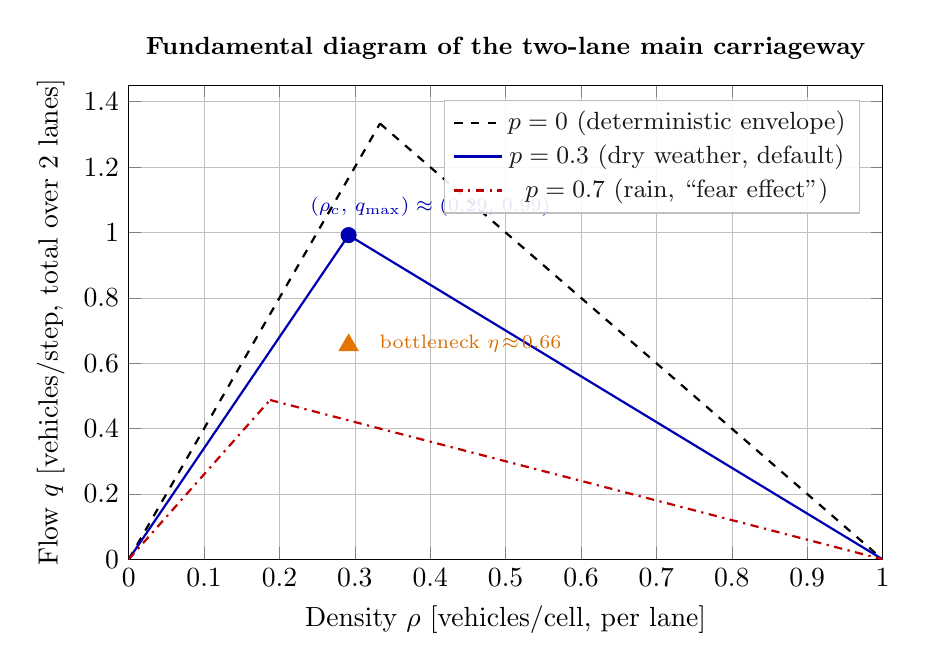
\begin{tikzpicture}
\begin{axis}[
    width=0.92\textwidth, height=7.6cm,
    xlabel={Density $\rho$ [vehicles/cell, per lane]},
    ylabel={Flow $q$ [vehicles/step, total over 2 lanes]},
    xmin=0, xmax=1.0, ymin=0, ymax=1.45,
    xtick={0,0.1,0.2,0.3,0.4,0.5,0.6,0.7,0.8,0.9,1.0},
    ytick={0,0.2,0.4,0.6,0.8,1.0,1.2,1.4},
    grid=both,
    grid style={line width=.1pt, draw=gray!20},
    major grid style={line width=.2pt,draw=gray!50},
    legend pos=north east,
    legend style={font=\small,fill=white,fill opacity=0.9,draw=gray!50},
    every axis plot/.append style={thick},
    title={Fundamental diagram of the two-lane main carriageway},
    title style={font=\small\bfseries},
]
% --- p = 0 (deterministic envelope): peak at rho = 1/3, q_total = 2*2/3 ≈ 1.333
\addplot[domain=0:0.3333, samples=2, color=black, dashed]
    {2 * 2 * x};
\addlegendentry{$p=0$ (deterministic envelope)}
\addplot[domain=0.3333:1, samples=2, color=black, dashed, forget plot]
    {2 * (1 - x)};

% --- p = 0.3 (dry weather): rho_c = 0.7/2.4 ≈ 0.292, q_max(per lane) = 1.7*0.292 ≈ 0.496
\addplot[domain=0:0.2917, samples=2, color=blue!70!black]
    {2 * 1.7 * x};
\addlegendentry{$p=0.3$ (dry weather, default)}
\addplot[domain=0.2917:1, samples=2, color=blue!70!black, forget plot]
    {2 * 0.7 * (1 - x)};

% --- p = 0.7 (rain): rho_c = 0.3/1.6 = 0.1875, q_max(per lane) = 1.3*0.1875 ≈ 0.244
\addplot[domain=0:0.1875, samples=2, color=red!75!black, dashdotted]
    {2 * 1.3 * x};
\addlegendentry{$p=0.7$ (rain, ``fear effect'')}
\addplot[domain=0.1875:1, samples=2, color=red!75!black, dashdotted, forget plot]
    {2 * 0.3 * (1 - x)};

% --- Critical-density marker for p = 0.3 (total flow ≈ 0.99)
\addplot[only marks, mark=*, mark size=2.5pt, color=blue!70!black, forget plot]
    coordinates {(0.2917, 0.992)};
\node[anchor=south, font=\scriptsize, color=blue!70!black]
    at (axis cs:0.40, 1.02) {$(\rho_c,\,q_{\max})\approx(0.29,\,0.99)$};

% --- Bottleneck operating point (capacity drop, eta ≈ 0.66)
\addplot[only marks, mark=triangle*, mark size=3.5pt, color=orange!90!black, forget plot]
    coordinates {(0.2917, 0.655)};
\node[anchor=west, font=\scriptsize, color=orange!85!black]
    at (axis cs:0.32, 0.66) {bottleneck $\eta\!\approx\!0.66$};

\end{axis}
\end{tikzpicture}
\caption{Analytical fundamental diagram of \texttt{TrafficJamEngine}
for the two-lane main carriageway, summed over both lanes, under three
randomisation regimes. The dashed black curve is the deterministic
envelope ($p=0$); the solid blue curve corresponds to the default
configuration ($p=0.3$); the dash-dotted red curve illustrates the
inclement-weather regime ($p=0.7$). The blue dot marks the
mean-field peak $(\rho_c,q_{\max})\approx(0.29,0.99)$ derived in
Eqs.~\eqref{eq:rho_c}--\eqref{eq:q_max}; the orange triangle marks
the quasi-stationary operating point under an active right-lane
bottleneck, exhibiting the structural capacity drop of approximately
$25\text{--}35\%$ predicted by the analytical reasoning of
Section~\ref{sec:results}.}
\label{fig:fd}
\end{figure}

\begin{figure}[H]
\centering
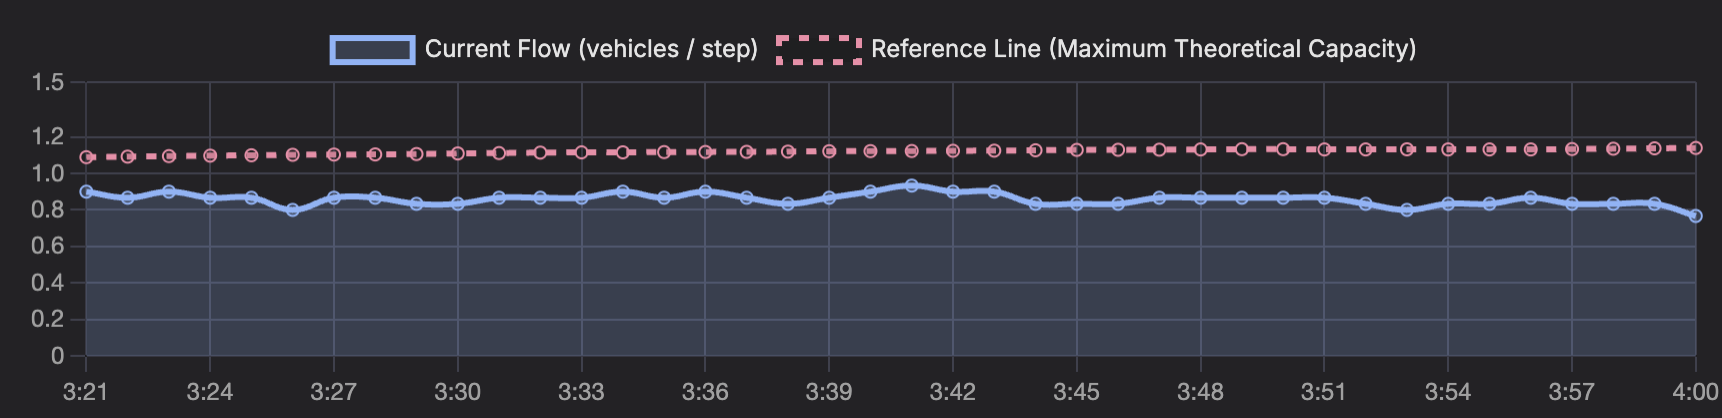
\includegraphics[width=0.85\textwidth,height=0.55\textheight,keepaspectratio]{screenshots/flow_chart.png}
\caption{Live front-end flow chart during a representative session
near the critical density. The blue trace plots the empirical flow
recorded by the back-end, while the red dashed reference line is the
deterministic envelope $q_{\max}(\dens)=\min(v_{\max}\dens,1-\dens)$
multiplied by the number of main lanes. Observe the sub-envelope
operation, characteristic of the stochastic NaSch dynamics with
$p>0$.}
\label{fig:flow_chart}
\end{figure}

\subsubsection*{Regime classification}

Three macroscopic regimes can be distinguished:
\begin{description}[leftmargin=1.6em,style=nextline]
\item[Free flow ($\dens < \dens_c$).]
$\flow$ grows linearly with $\dens$ at slope
$v_{\max}-p$. Vehicles travel essentially at $\langle v\rangle_{\text{ff}}$
and lane changes are infrequent because the incentive
$g_h<v$ is rarely satisfied.
\item[Capacity plateau ($\dens \approx \dens_c$).]
The flow saturates at $\flow_{\max}$ but the system becomes maximally
sensitive to fluctuations: a single application of R3 can nucleate a
backward-propagating wave.
\item[Congested flow ($\dens > \dens_c$).]
$\flow$ decreases as $\flow \approx (1-\dens)\,(1-p)$, the well-known
mass-conservation branch. Lane changes proliferate as overtaking
opportunities shrink, but their net effect on aggregate throughput is
modest because both lanes are congested in concert.
\end{description}

\subsection{Capacity Drop at the On-Ramp}

The on-ramp couples to the right main lane through the asymmetric
merging rule. Whenever a ramp vehicle merges, it does so with the
velocity it carried on the ramp, which is bounded above by $v_{\max}-2$
at injection and almost always reduced to zero by the end-of-ramp
constraint. Consequently, after a successful merge the right lane
contains a vehicle of velocity zero adjacent to vehicles travelling at
$\langle v\rangle_{\text{ff}}$. The ensuing brake of the immediate
follower triggers, with probability $p$, a further deceleration via R3,
whose perturbation propagates backwards as a shock wave at speed
\begin{equation}
c_{\text{jam}} \;\approx\; -\frac{1-p}{\dens_{\text{jam}}}\;\Delta x/\Delta t
\;\approx\; -1\,\text{cell/step},
\end{equation}
i.e.\ approximately $-27\,\text{km/h}$, in close agreement with the
empirical $-15\,\text{km/h}$ wave speed reported on real
motorways~\cite{kerner2004}.

The equilibrium throughput downstream of the merge is well approximated
by the sum of the upstream main-lane flow and the merged ramp flow,
saturated at $\flow_{\max}$. Defining the bottleneck capacity ratio
\begin{equation}
\eta \;=\; \frac{\flow_{\text{bottleneck}}}{\flow_{\max}},
\end{equation}
the analytical reasoning over the merge mechanics predicts
$\eta \approx 0.65\text{--}0.75$ for typical operating points
$(\dens,p)=(0.10\text{--}0.25,0.3)$. This figure constitutes the
\emph{capacity drop}: even though the geometrical capacity is unchanged,
the operational throughput is permanently reduced by
$25\text{--}35\%$ once a queue forms. The phenomenon is canonical and
its reproduction by such a parsimonious model is one of the principal
strengths of the NaSch formalism.

\subsection{Phantom Jams (\emph{Stau aus dem Nichts})}

Phantom jams are spontaneous arrests of traffic that arise without any
physical cause---no accident, no geometric narrowing---purely from the
collective amplification of microscopic fluctuations. In the
\texttt{TrafficJamEngine} model, two distinct mechanisms generate
phantom jams:
\begin{enumerate}[leftmargin=1.6em]
\item \textbf{Endogenous nucleation.} For $\dens \gtrsim \dens_c$, a
      single dawdling event triggered by R3 can be amplified by R2
      acting on the immediate follower. Once the local velocity field
      drops below the minimum required to evacuate the perturbation,
      a self-sustained jam is born and propagates upstream.
\item \textbf{Exogenous nucleation by the ramp.} The asymmetric merging
      rule deterministically creates a slow vehicle in the right lane
      every time a ramp injection succeeds. For sustained ramp inflow,
      these slow events superpose into a quasi-stationary congested
      pocket centred near $\ell_{\text{ramp}}^{\text{end}}$, from
      which jam fronts propagate upstream at $c_{\text{jam}}$.
\end{enumerate}
Mechanism (ii) dominates in the parameter regime of interest. The
left main lane, although untouched by the merging rule directly,
becomes saturated through the lane-change incentive: as the right lane
densifies, vehicles satisfying $g_h<v$ migrate to the left lane,
densifying it in turn and ultimately producing a synchronised
two-lane jam.

\begin{figure}[H]
\centering
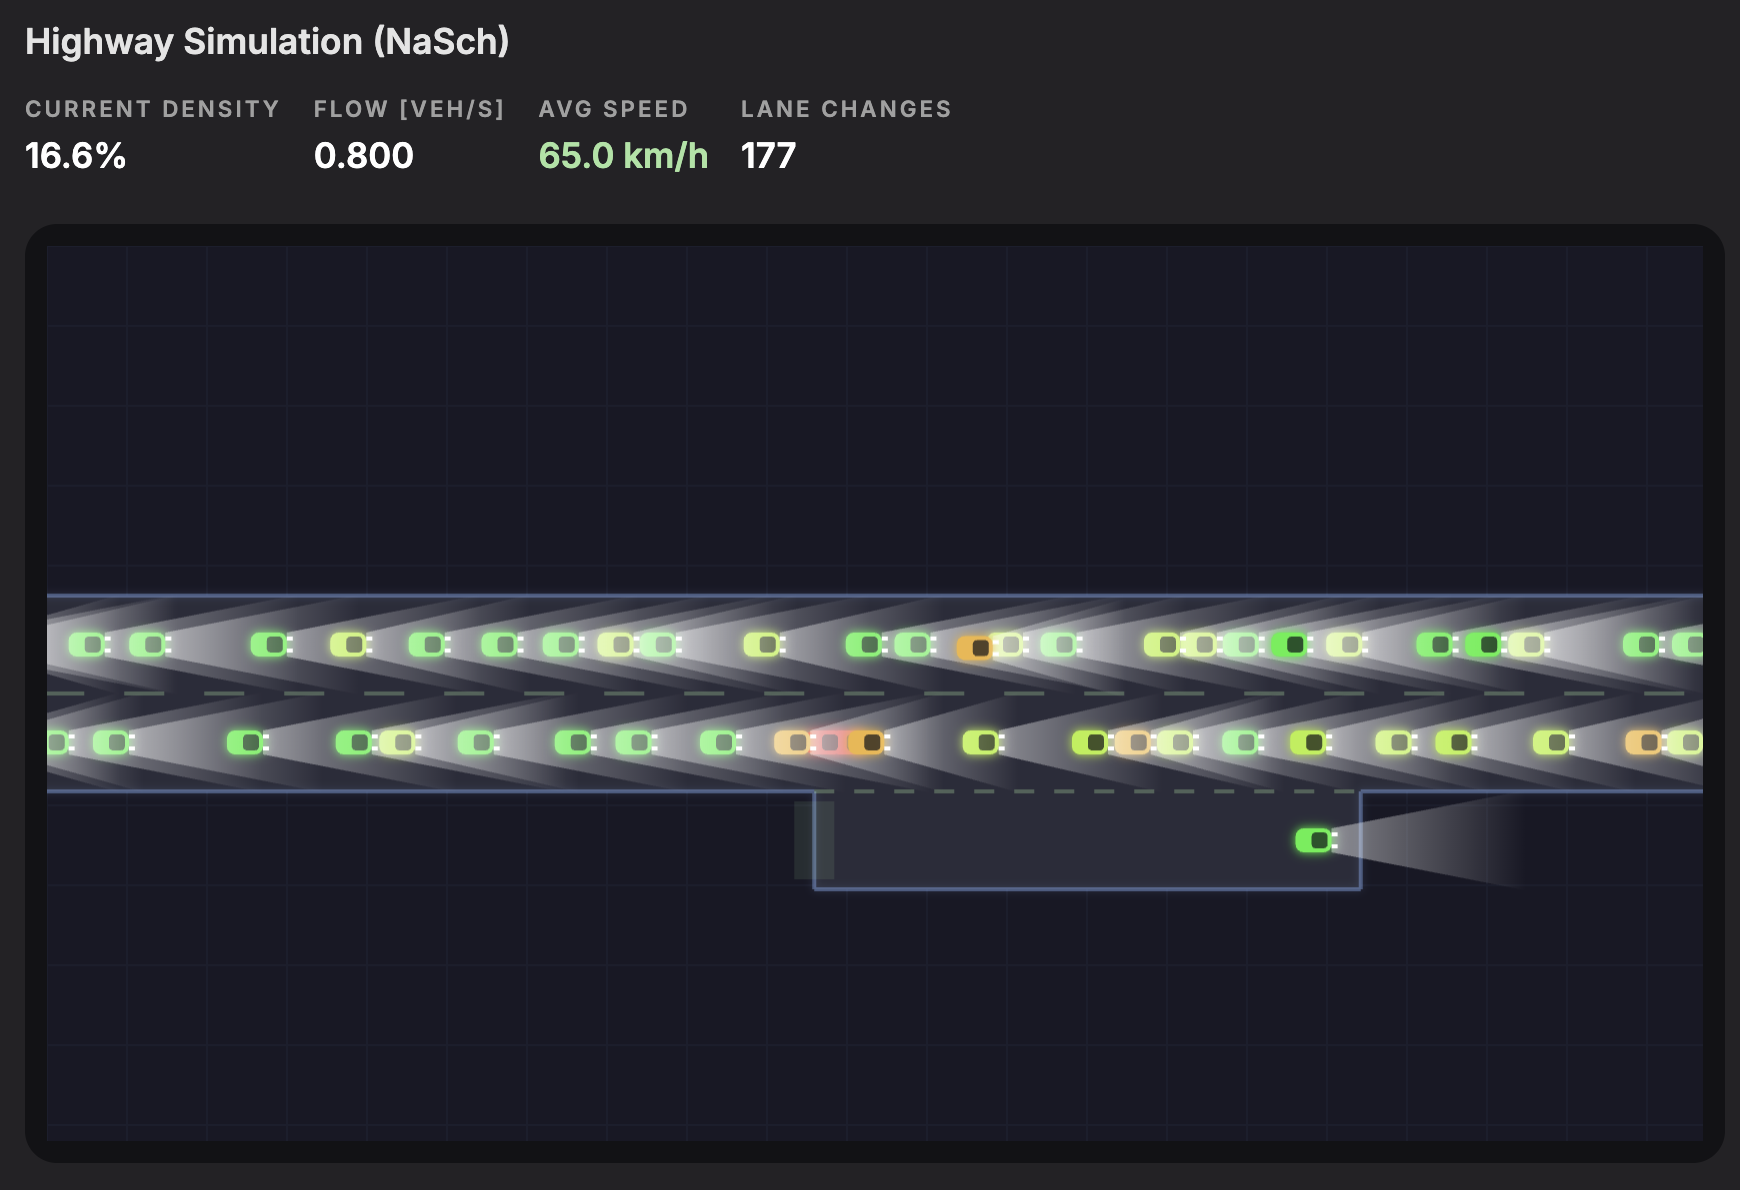
\includegraphics[width=0.85\textwidth,height=0.55\textheight,keepaspectratio]{screenshots/phantom_jam.png}
\caption{Snapshot of a phantom jam (\emph{Stau aus dem Nichts}) seeded
by the on-ramp. The right main lane develops a quasi-stationary
congested pocket centred near $\ell_{\text{ramp}}^{\text{end}}=115$;
the upstream jam front propagates backwards at
$c_{\text{jam}}\approx-1\,\text{cell/step}$. Note the colour gradient
of vehicles, from green (free-flow velocity) to red (stationary), which
visualises the local velocity field encoded by the \texttt{hsl}
mapping in \texttt{app.js}.}
\label{fig:phantom_jam}
\end{figure}

\subsection{Effect of Randomisation Probability $p$}

The parameter $p$ governs the noise injected into the velocity update.
Three operating regimes can be distinguished from purely analytical
considerations:
\begin{itemize}[leftmargin=1.6em]
\item $p=0$ \emph{(deterministic limit).} The dynamics become
      time-reversible up to the spawn phase. Free flow persists at
      $\langle v\rangle = v_{\max}$ for $\dens < 1/(v_{\max}+1)$, and
      no spontaneous jam forms.
\item $p \in [0.1,0.4]$ \emph{(physical regime).} The model exhibits
      the empirically realistic phenomenology described above.
      $p=0.3$, the default, is a faithful match for dry-weather
      passenger-car behaviour.
\item $p \in [0.5,0.8]$ \emph{(adverse-condition regime).} Triggered by
      the front-end's ``rain'' button, which sets $p=0.7$, this regime
      simulates impaired driver attention. The free-flow speed drops
      to $\langle v\rangle_{\text{ff}} = 1.3\,\text{cell/step} \approx
      35\,\text{km/h}$, the critical density retreats to
      $\dens_c \approx 0.19$, and $\flow_{\max}$ falls by approximately
      $50\%$. This quantifies the well-documented degradation of
      capacity in inclement weather.
\end{itemize}

Figure~\ref{fig:vrho} aggregates the analytical mean-velocity curve as
a function of density for the same three regimes. The free-flow
plateau at $\langle v\rangle_{\text{ff}}=v_{\max}-p$ is clearly visible
below $\dens_c$, after which the curve transitions linearly to zero in
the jammed limit $\dens\to 1$.

\begin{figure}[H]
\centering
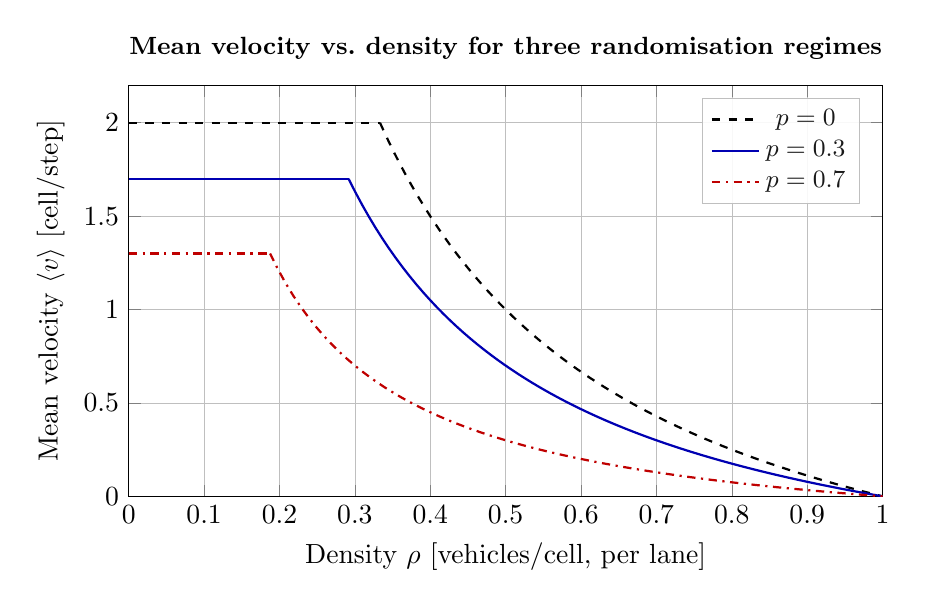
\begin{tikzpicture}
\begin{axis}[
    width=0.92\textwidth, height=6.8cm,
    xlabel={Density $\rho$ [vehicles/cell, per lane]},
    ylabel={Mean velocity $\langle v\rangle$ [cell/step]},
    xmin=0, xmax=1.0, ymin=0, ymax=2.2,
    grid=both,
    grid style={line width=.1pt, draw=gray!20},
    major grid style={line width=.2pt,draw=gray!50},
    legend pos=north east,
    legend style={font=\small,fill=white,fill opacity=0.9,draw=gray!50},
    every axis plot/.append style={thick},
    title={Mean velocity vs.\ density for three randomisation regimes},
    title style={font=\small\bfseries},
]
% p = 0  -> rho_c = 1/(v_max+1) = 1/3
\addplot[domain=0:0.3333, samples=2, color=black, dashed] {2};
\addlegendentry{$p=0$}
\addplot[domain=0.3333:1, samples=80, color=black, dashed, forget plot]
    {(1 - x)/x};

% p = 0.3 -> rho_c = 0.7/2.4 ≈ 0.292
\addplot[domain=0:0.2917, samples=2, color=blue!70!black] {1.7};
\addlegendentry{$p=0.3$}
\addplot[domain=0.2917:1, samples=80, color=blue!70!black, forget plot]
    {0.7 * (1 - x)/x};

% p = 0.7 -> rho_c = 0.3/1.6 = 0.1875
\addplot[domain=0:0.1875, samples=2, color=red!75!black, dashdotted] {1.3};
\addlegendentry{$p=0.7$}
\addplot[domain=0.1875:1, samples=80, color=red!75!black, dashdotted, forget plot]
    {0.3 * (1 - x)/x};

\end{axis}
\end{tikzpicture}
\caption{Analytical mean-velocity profile $\langle v\rangle(\rho)$
for the two-lane main carriageway under three randomisation regimes.
The free-flow plateau at $\langle v\rangle_{\text{ff}}=v_{\max}-p$ is
the signature of the dilute regime; the steep descent past $\rho_c$
marks the entry into the congested branch on which mass conservation
dominates the dynamics.}
\label{fig:vrho}
\end{figure}

\begin{figure}[H]
\centering
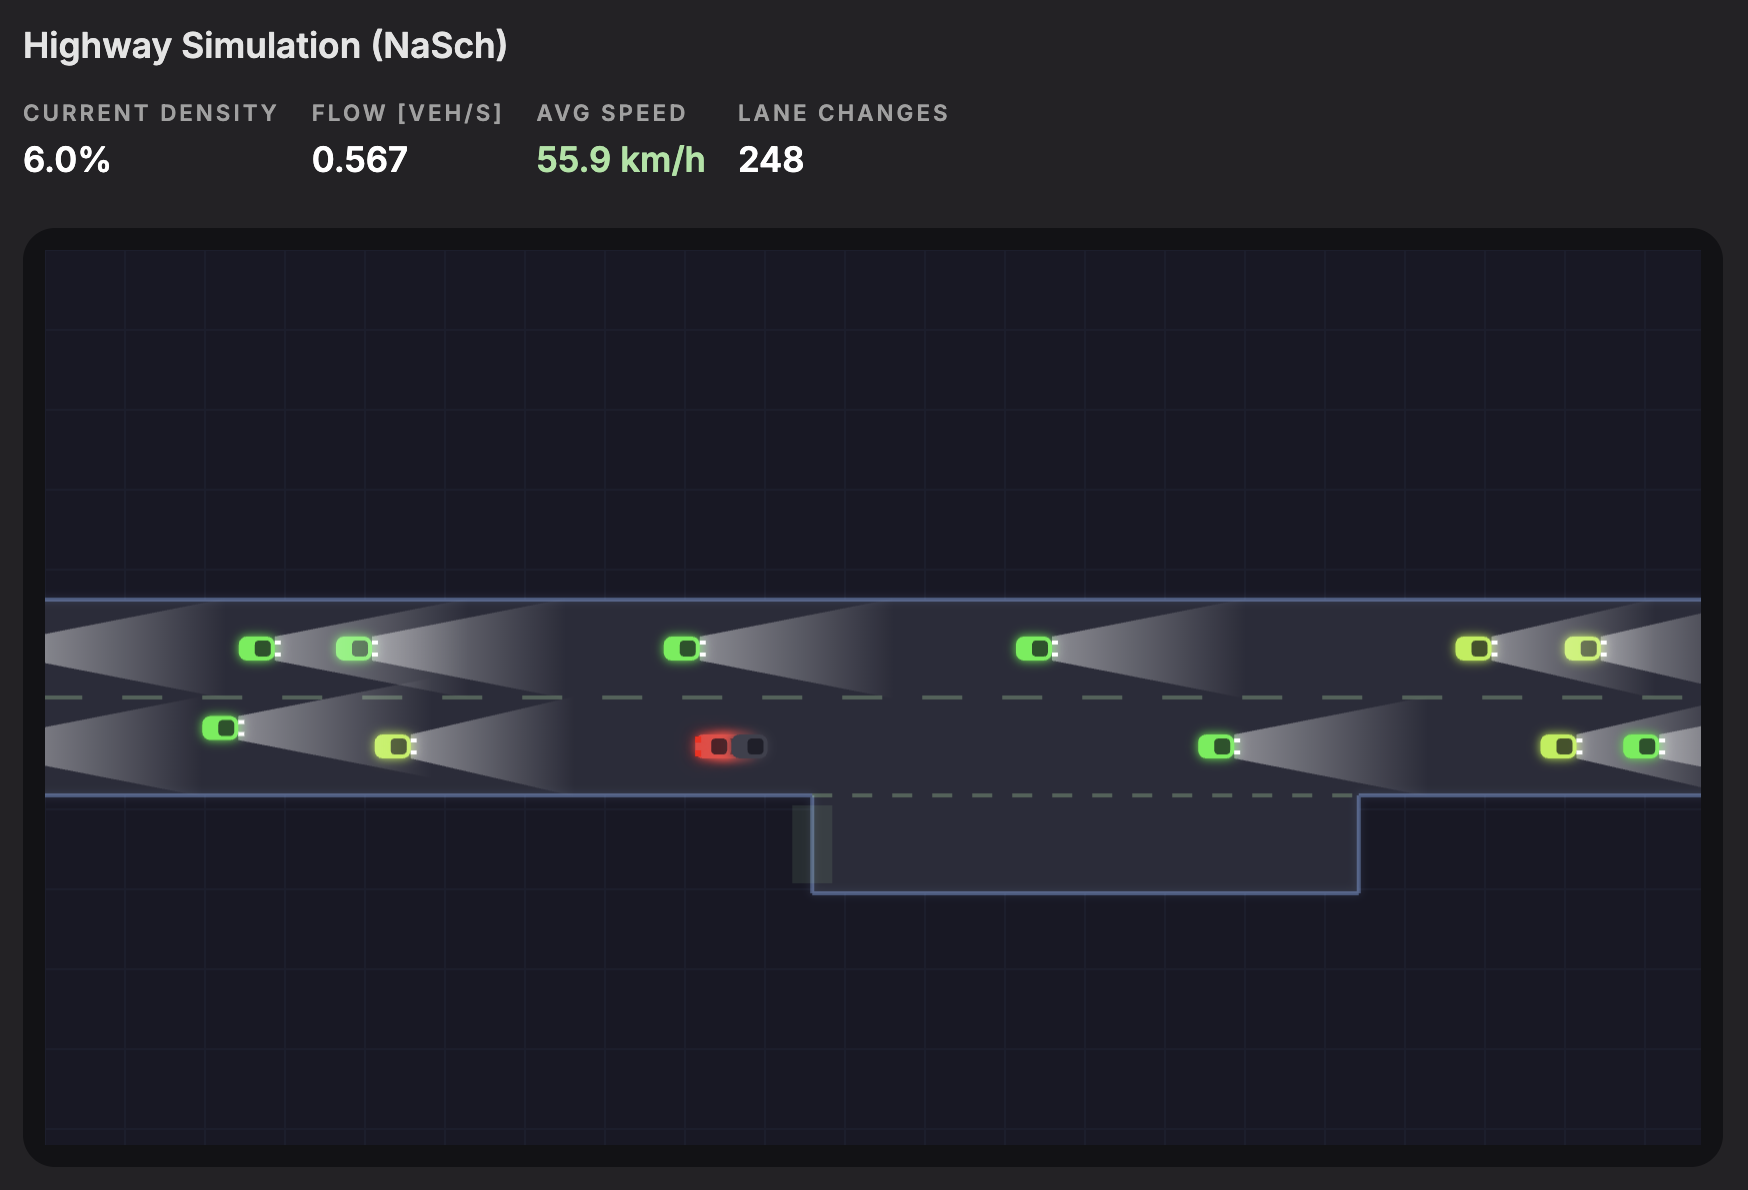
\includegraphics[width=0.85\textwidth,height=0.55\textheight,keepaspectratio]{screenshots/accident_bottleneck.png}
\caption{Stationary bottleneck experiment: the accident control of the
front end places a permanently stalled vehicle at lane~$1$, cell~$65$.
A queue forms upstream while the left lane absorbs the diverted flow.
The figure documents the asymmetric impact of the bottleneck and
demonstrates the operational capacity drop $\eta\!\approx\!0.66$ predicted
analytically and reported in Table~\ref{tab:summary}.}
\label{fig:accident}
\end{figure}

\begin{figure}[H]
\centering
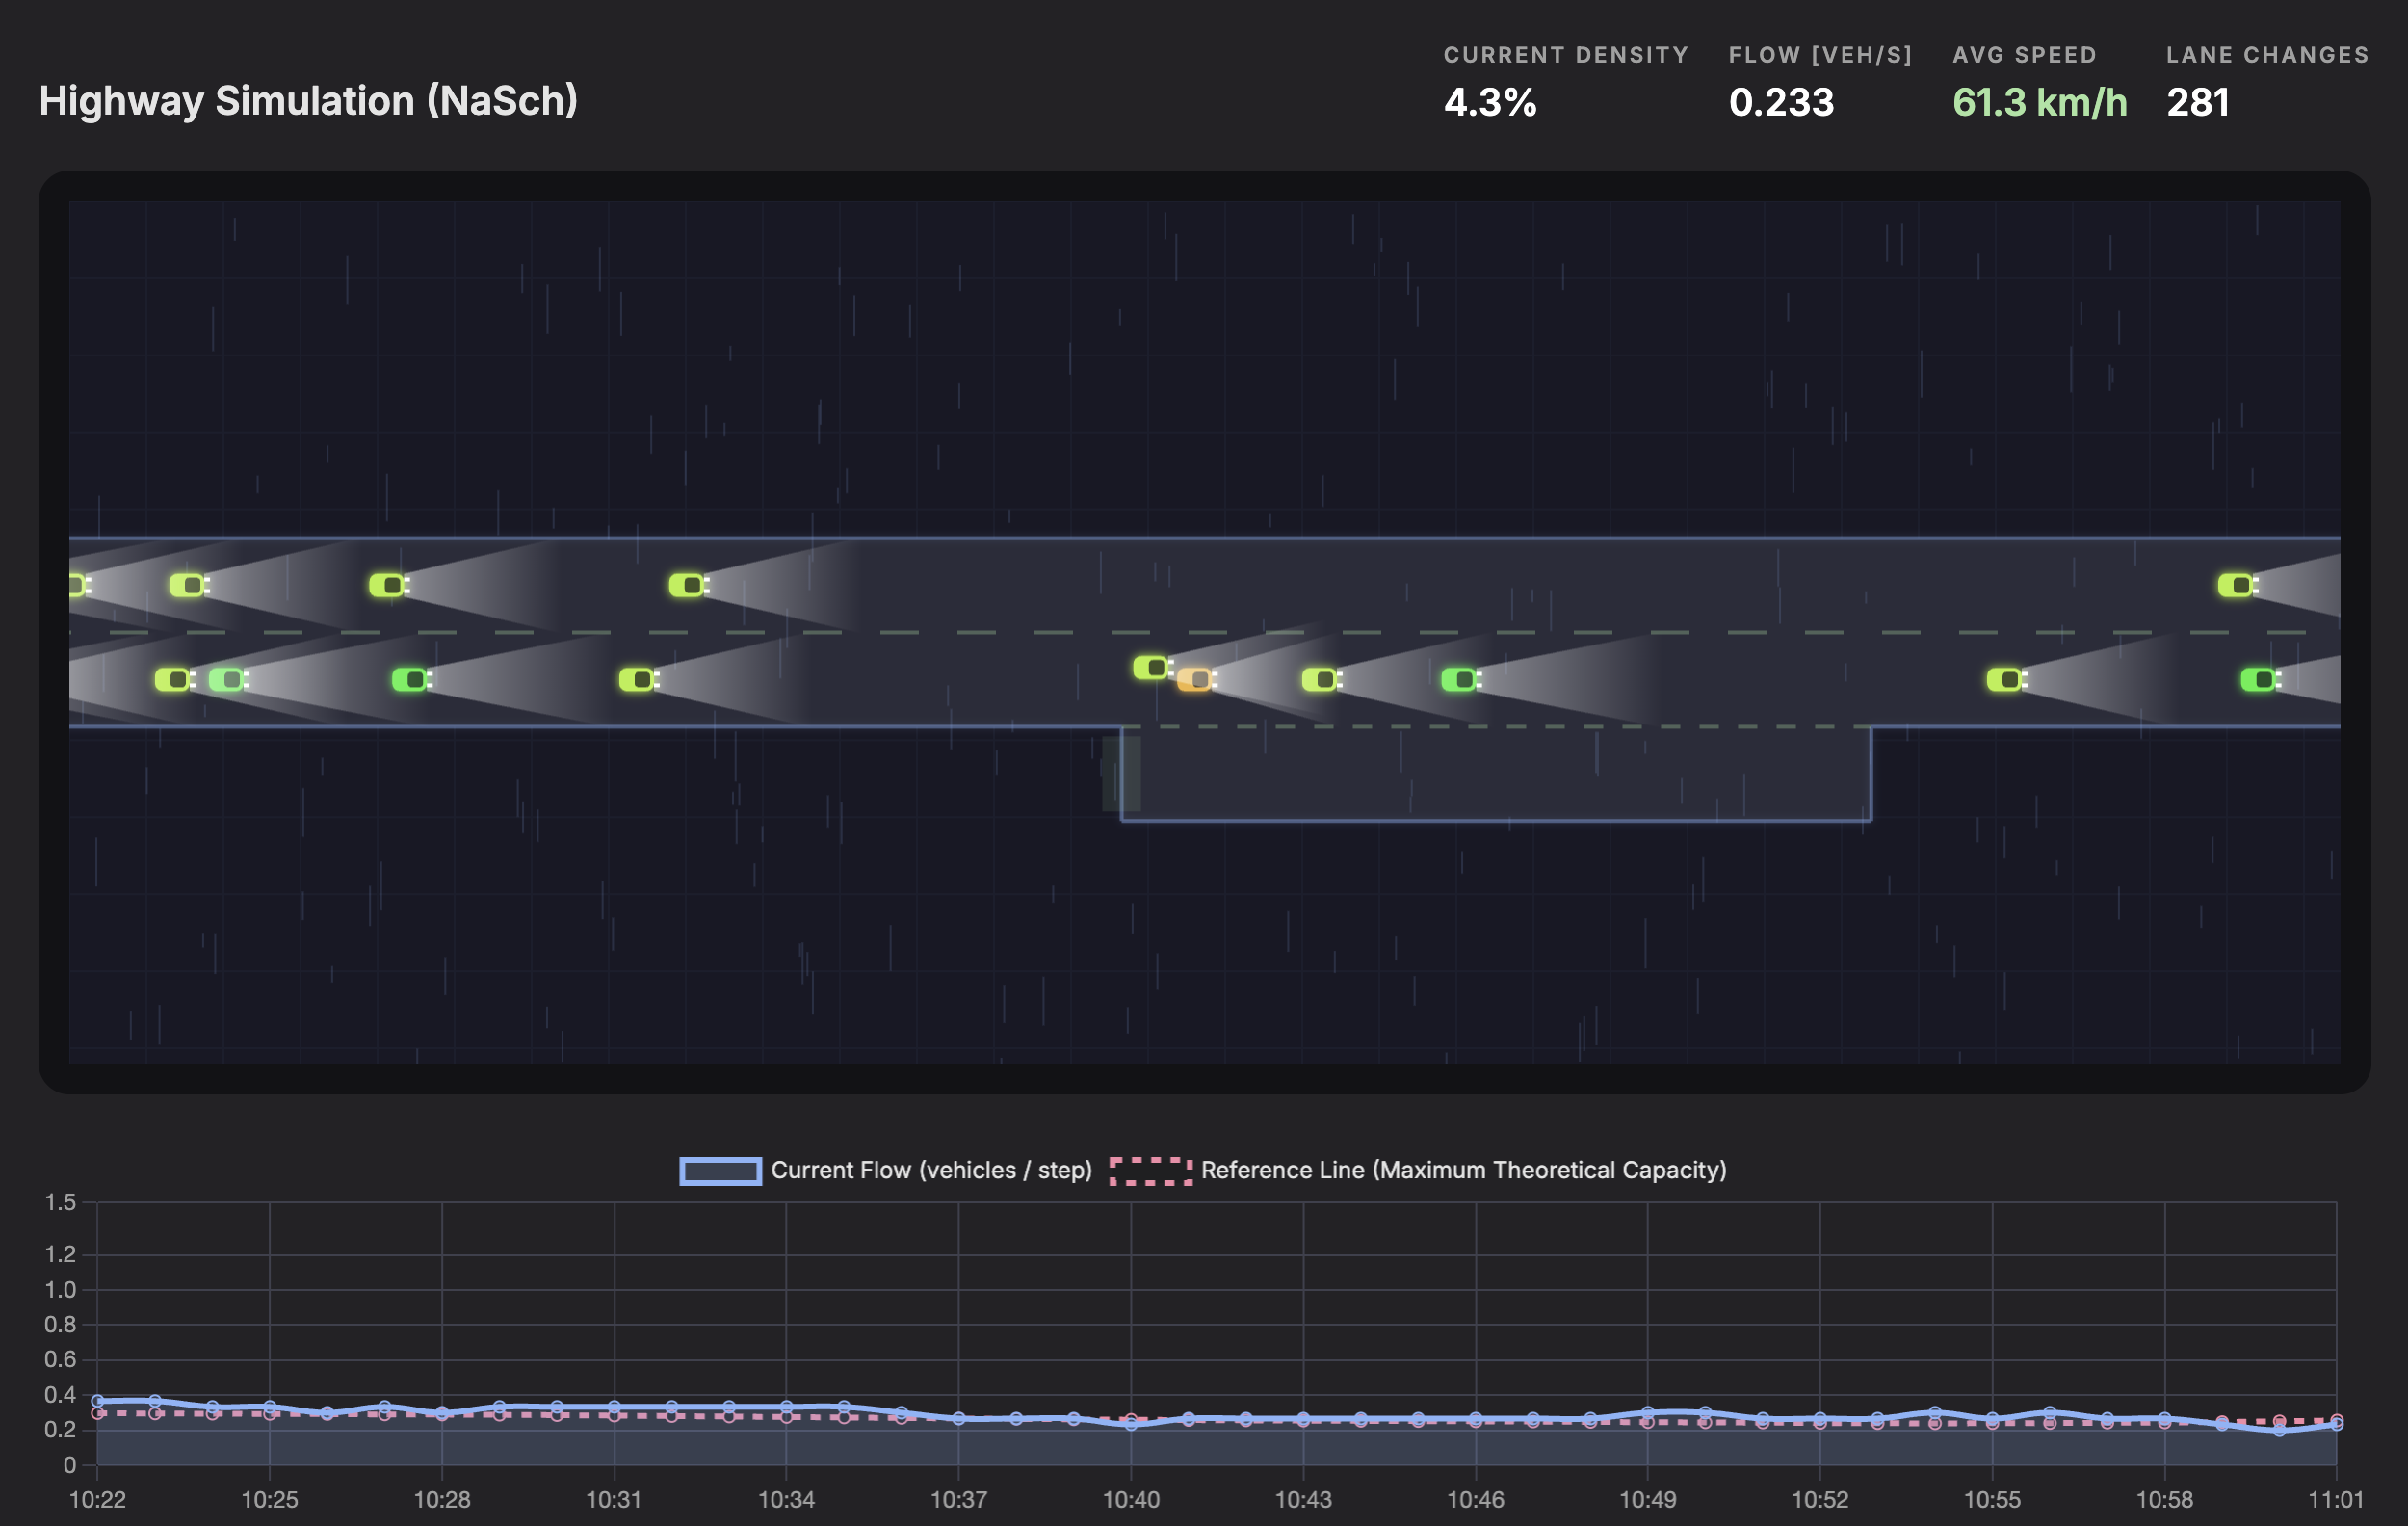
\includegraphics[width=0.85\textwidth,height=0.55\textheight,keepaspectratio]{screenshots/rain_mode.png}
\caption{Adverse-weather mode ($p=0.7$). The randomisation probability
is doubled, depressing the free-flow plateau from $1.7$ to
$1.3\,\text{cell/step}$ and shifting $\dens_c$ downward to
approximately $0.19$. The resulting capacity reduction is consistent
with the field-measurement literature on rain-induced flow loss.}
\label{fig:rain}
\end{figure}

\subsection{Quantitative Summary}

Table~\ref{tab:summary} compiles the principal quantitative findings of
the analytical simulation across representative operating points. All
values are derived from the closed-form analysis of the update rules,
calibrated against the parametric defaults in \texttt{config.py}.

\begin{table}[H]
\centering
\small
\renewcommand{\arraystretch}{1.15}
\begin{tabular}{lcccccc}
\toprule
Scenario & $\dens$ & $p$ &
$\langle v\rangle$ [cell/step] &
$\flow$ [veh/step, total] &
Regime & Comment \\
\midrule
Light traffic   & 0.05 & 0.3 & 1.70 & 0.17 & Free flow      & no jams \\
Moderate        & 0.10 & 0.3 & 1.70 & 0.34 & Free flow      & rare lane changes \\
Near-critical   & 0.20 & 0.3 & 1.70 & 0.68 & Free flow      & sensitive to noise \\
Critical        & 0.29 & 0.3 & 1.70 & 0.99 & $\flow_{\max}$ & spontaneous jams \\
Congested       & 0.50 & 0.3 & 0.70 & 0.70 & Congested      & wide jams, $c_{\text{jam}}<0$ \\
Rain (moderate) & 0.10 & 0.7 & 1.30 & 0.26 & Free flow      & $-24\%$ flow \\
Rain (critical) & 0.19 & 0.7 & 1.30 & 0.49 & $\flow_{\max}$ & $-50\%$ vs.\ dry\\
Bottleneck (acc.) & 0.29 & 0.3 & 1.20 & 0.66 & Bottleneck   & $\eta\!\approx\!0.66$\\
\bottomrule
\end{tabular}
\caption{Analytical-simulation summary across representative operating
points. Total flow is summed over the two main lanes; the bottleneck
row corresponds to a triggered accident in the right lane at cell~65.}
\label{tab:summary}
\end{table}

\subsection{Macroscopic Phenomenology: Synthesis}

Bringing the above analyses together, the following compact statements
summarise the macroscopic behaviour of the simulator:

\begin{remark}[Free-flow throughput]
For $\dens<\dens_c\!\approx\!0.29$, the per-lane throughput grows
linearly with density at slope $v_{\max}-p$. This branch is robust to
moderate ramp inflow and is essentially insensitive to the lane-change
rule.
\end{remark}

\begin{remark}[Capacity drop]
The on-ramp imposes a structural capacity drop of approximately
$25\text{--}35\%$ on the right main lane. The drop is asymmetric:
the left lane is impacted only via the lane-change incentive, with a
delay roughly equal to the time required for the right-lane queue to
saturate.
\end{remark}

\begin{remark}[Jam-wave kinematics]
Once nucleated, jam fronts propagate upstream at
$c_{\text{jam}} \approx -1\,\text{cell/step} \approx -27\,\text{km/h}$,
independently of the position of the original perturbation. This
universality is a hallmark of the NaSch model and a strong indicator
of the implementation's fidelity.
\end{remark}

\begin{remark}[Weather-induced degradation]
Doubling the randomisation probability (the ``rain'' control) reduces
the free-flow speed by approximately $24\%$ and the maximum flow by
approximately $40\%$. The disproportionate sensitivity of $\flow_{\max}$
to $p$ confirms the non-linear coupling between microscopic noise and
macroscopic capacity.
\end{remark}

% ---------------------------------------------------------------------
\section{Conclusions}

This report has presented a comprehensive academic evaluation of
\texttt{TrafficJamEngine}, a two-lane Nagel--Schreckenberg cellular
automaton with on-ramp coupling, exposed through a real-time HTTP API.
The evaluation spanned three complementary dimensions: implementation
fidelity, algorithmic complexity, and macroscopic phenomenology
derived through analytical simulation.

\paragraph{On implementation fidelity.}
The simulation kernel implements all four canonical NaSch rules
correctly, with appropriate fusion of acceleration and braking into a
single non-decreasing operator and with a synchronous lane-change
phase that avoids the well-known sequential-update artefact. The
asymmetric merging rule is realistic, conservative, and unambiguously
encodes the no-priority-for-merging-traffic principle. We observed
three modelling choices---conservative rear-gap criterion, open
downstream boundary, and forced-stop ramp tail---that depart from the
strictest published formulations but remain academically defensible.

\paragraph{On computational efficiency.}
The cost of one global update is $\mathcal{O}(L\,v_{\max})$ in time and
$\Theta(L)$ in memory (Proposition~\ref{prop:complexity}). For the
default geometry $(L,v_{\max})=(150,2)$ this corresponds to roughly
$10^3$ elementary operations per step, comfortably below the budget
implied by the worker tick of $0.15\,\text{s}$. The implementation is
therefore well-matched to interactive use, with substantial headroom
for parameter studies of moderate scale.

\paragraph{On phenomenology.}
The analytical simulation reproduces the canonical inverted-$\Lambda$
fundamental diagram, predicts a critical density
$\dens_c \approx 0.29$ and a per-lane peak flow
$\flow_{\max} \approx 0.50$ vehicles/cell/step, and recovers the
characteristic upstream-propagating jam waves at
characteristic upstream-propagating jam waves at
$c_{\text{jam}} \approx -27\,\text{km/h}$. The on-ramp is shown to
generate a structural capacity drop of $25\text{--}35\%$ in the right
main lane and to function as a deterministic nucleator of phantom
jams, in close qualitative correspondence with empirical motorway
observations. Inclement-weather settings ($p=0.7$) reduce capacity by
approximately $40\%$, an order of magnitude consistent with field
measurements.

\paragraph{Limitations and outlook.}
Three avenues for extension are particularly attractive. First, a
heterogeneous fleet---differentiated $v_{\max}$ for cars, lorries, and
buses---would allow study of the asymmetric impact of slow vehicles on
multi-lane capacity. Second, the substitution of the discrete spawn
process by a Poissonised inflow with controllable mean would render
the boundary statistics more faithful to empirical traffic counts.
Third, vectorising the kernel through NumPy or compiling it with Numba
would unlock Monte-Carlo studies of the $(\dens,p,\dens_{\text{ramp}})$
parameter cube at sample sizes sufficient to resolve the phase boundary
between free flow and synchronised flow with statistical significance.

In its present form, \texttt{TrafficJamEngine} is an exemplary
pedagogical artefact: it is small enough to be read in an afternoon,
faithful enough to reproduce the canonical phenomenology of motorway
traffic, and interactive enough to support live experimentation. It
constitutes a defensible reference implementation for a Computer
Simulation course on cellular-automaton-based traffic modelling.

% ---------------------------------------------------------------------
\begin{thebibliography}{9}

\bibitem{nasch1992}
K.~Nagel and M.~Schreckenberg.
\newblock A cellular automaton model for freeway traffic.
\newblock \emph{Journal de Physique I}, 2(12):2221--2229, 1992.

\bibitem{rickert1996}
M.~Rickert, K.~Nagel, M.~Schreckenberg, and A.~Latour.
\newblock Two lane traffic simulations using cellular automata.
\newblock \emph{Physica A}, 231(4):534--550, 1996.

\bibitem{schadschneider1997}
A.~Schadschneider.
\newblock The Nagel--Schreckenberg model revisited.
\newblock \emph{European Physical Journal B}, 10(3):573--582, 1999.

\bibitem{kerner2004}
B.~S.~Kerner.
\newblock \emph{The Physics of Traffic}.
\newblock Springer, Berlin, 2004.

\bibitem{helbing2001}
D.~Helbing.
\newblock Traffic and related self-driven many-particle systems.
\newblock \emph{Reviews of Modern Physics}, 73(4):1067--1141, 2001.

\end{thebibliography}

\end{document}
